\section{Server Konfiguration}
\subsection{Screenshots}
\begin{minipage}[t]{\textwidth}
	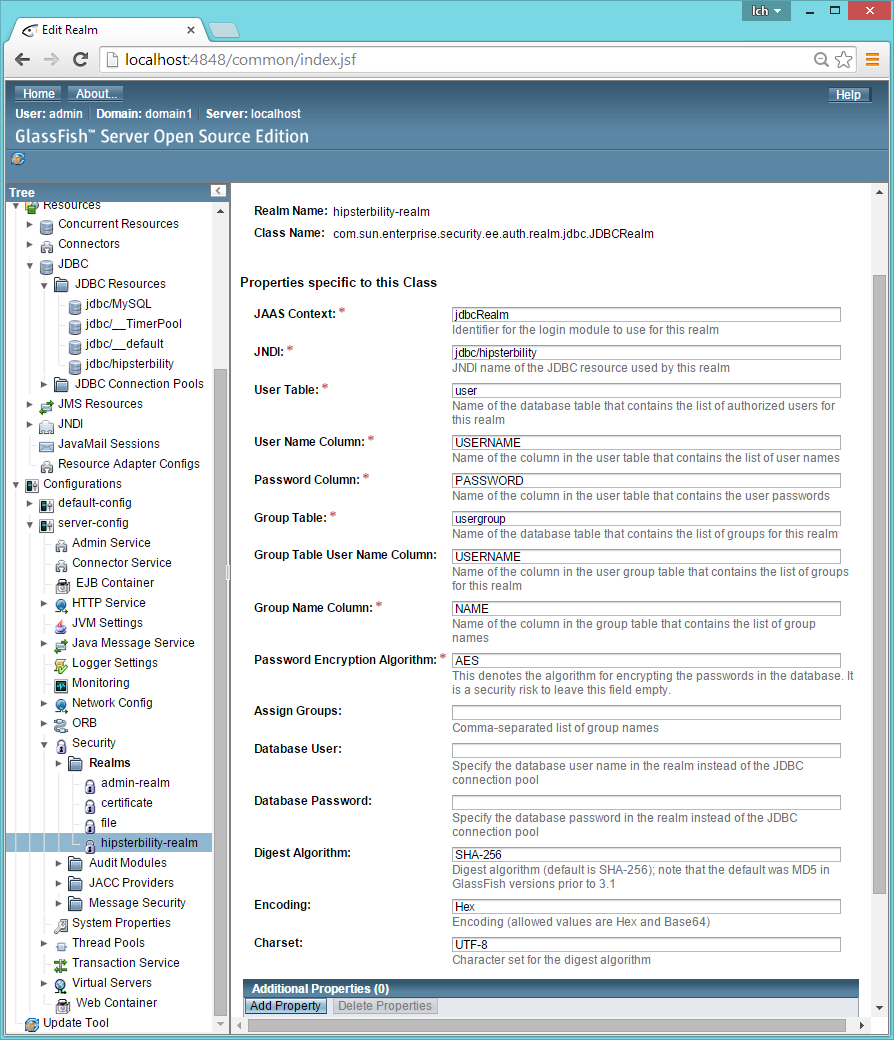
\includegraphics[width = \linewidth]{img/screenshot_realm.png}
	\captionof{figure}{Screenshot der Security-Realm Konfiguration des Glassfish Servers}
	\label{fig:realm_screenshot}
\end{minipage}

\newpage
\subsection{Glassfish Befehle}

\lstinputlisting[caption={Erstellen eines Glassfish Security Realms mit dem \enquote{asadmin} Werkzeug.},language=bash, firstline=2,label=lst:asadmin_create_realm]{../../UsabilityToolkit/HipsterbilityServer/src/main/scripts/glassfish-create.txt}


\subsection{Konfigurationsdateien}

\lstinputlisting[caption={glassfish-resources.xml zum Erzeugen eines JDBC Resource-Pools und einer JDBC Ressource},language=XML,label=lst:glassfish-resources_xml]{../../UsabilityToolkit/HipsterbilityServer/src/main/scripts/glassfish-resources.xml}

\lstinputlisting[caption={glassfish-web.xml JSP Konfiguration und Mapping von SecurityRealm Rollen.},language=XML, label=lst:glassfish-web_xml]{../../UsabilityToolkit/HipsterbilityServer/src/main/webapp/WEB-INF/glassfish-web.xml}

\subsection{Scriptdateien}
\subsubsection{Befehlsdateien}
\lstinputlisting[caption={glassfish-create.txt Befehle zu erzeugen von Ressourcen.},language=bash,label=lst:glassfish-create]{../../UsabilityToolkit/HipsterbilityServer/src/main/scripts/glassfish-create.txt}

\lstinputlisting[caption={glassfish-delete.txt Befehle zum Löschen von Ressourcen.},language=bash,label=lst:glassfish-delete]{../../UsabilityToolkit/HipsterbilityServer/src/main/scripts/glassfish-delete.txt}

\subsubsection*{Windows}
\lstinputlisting[caption={glassfish-create-resources.bat},language=bash,label=lst:glassfish-create-resources_bat]{../../UsabilityToolkit/HipsterbilityServer/src/main/scripts/glassfish-create-resources.bat}

\lstinputlisting[caption={glassfish-delete-resources.bat},language=bash,label=lst:glassfish-delete-resources_bat]{../../UsabilityToolkit/HipsterbilityServer/src/main/scripts/glassfish-delete-resources.bat}

\subsubsection*{Unix / Linux}

\lstinputlisting[caption={glassfish-create-resources.sh},language=bash,label=lst:glassfish-create-resources_sh]{../../UsabilityToolkit/HipsterbilityServer/src/main/scripts/glassfish-create-resources.sh}

\lstinputlisting[caption={glassfish-delete-resources.sh},language=bash,label=lst:glassfish-delete-resources_sh]{../../UsabilityToolkit/HipsterbilityServer/src/main/scripts/glassfish-delete-resources.sh}


\section{Serverkonfiguration}

\lstinputlisting[caption={persistence.xml (Datenbankverbindung)},language=XML, label=lst:persistence_xml]{../../UsabilityToolkit/HipsterbilityServer/src/main/resources/META-INF/persistence.xml}

\lstinputlisting[caption={web.xml (Servlet Konfiguration)},language=XML, label=lst:web_xml]{../../UsabilityToolkit/HipsterbilityServer/src/main/webapp/WEB-INF/web.xml}
